\documentclass[11pt]{article}
% Libraries.
\usepackage{amsmath}
\usepackage{amssymb}
\usepackage{pgfplots}
\usepackage{graphicx}
\usepackage{enumitem}
\usepackage{hyperref}
\usepackage{fancyhdr}
\usepackage{perpage}
\usepackage{float}
\usepackage{esint}
\usepackage{graphicx}
\graphicspath{ {./images/} }

% Property settings.
\MakePerPage{footnote}
\pagestyle{headings}

% Commands
\newcommand{\ti}[1]{\textit{#1}}
\newcommand{\tb}[1]{\textbf{#1}}
\newcommand{\mb}[1]{\mathbb{#1}}
\newcommand{\bx}[0]{\mathbf{x}}
\newcommand{\bv}[0]{\mathbf{v}}
\newcommand{\bw}[0]{\mathbf{w}}
\newcommand{\real}[0]{\mathbb{R}}
\newcommand{\under}[1]{\underline{#1}}
\newcommand{\proof}[0]{\textit{\underline{proof:} }}
\newcommand{\func}[3]{\tb{#1}: {#2} \rightarrow {#3} }
\newcommand{\vx}[0]{\tb{x}}
\newcommand{\vy}[0]{\tb{y}}
\newcommand{\vz}[0]{\tb{z}}
\newcommand{\vo}[0]{\tb{0}}
\newcommand{\va}[0]{\tb{a}}
\newcommand{\vb}[0]{\tb{b}}
\newcommand{\vc}[0]{\tb{c}}
\newcommand{\ve}[0]{\tb{e}}
\newcommand{\vm}[0]{\tb{m}}
\newcommand{\vh}[0]{\tb{h}}
\newcommand{\vf}[0]{\tb{F}}
\newcommand{\vi}[0]{\tb{i}}
\newcommand{\vj}[0]{\tb{j}}
\newcommand{\vk}[0]{\tb{k}}
\newcommand{\vg}[0]{\tb{G}}
\newcommand{\vn}[0]{\tb{n}}
\newcommand{\vu}[0]{\tb{u}}
\newcommand{\vL}[0]{\tb{L}}
\newcommand{\ff}[0]{\tb{f}}
\newcommand{\fg}[0]{\tb{g}}
\newcommand{\rational}[0]{\mathbb{Q}}
\newcommand{\p}[0]{\partial}
\newcommand{\qed}[0]{$\hfill\blacksquare$}
\newcommand{\qerat}{\tag*{$\blacksquare$}}
\newcommand{\lima}{\underset{\vx \rightarrow \va}{\lim}}
\usepackage{amsmath}% http://ctan.org/pkg/amsmath
\newcommand{\notimplies}{%
  \mathrel{{\ooalign{\hidewidth$\not\phantom{=}$\hidewidth\cr$\implies$}}}}
\newcommand{\q}[0]{\textcolor{red}{???}}

% Attr.
\title{CSC373 \\ Lecture Notes}
\author{Yuchen Wang}
\date{\today}

\begin{document}
    \maketitle
    \tableofcontents
    \newpage
\section{Divide \& Conquer}
\paragraph{General framework}
\begin{enumerate}
	\item Break (a large chunk of) a problem into smaller subproblems of the same type
	\item Solve each subproblem recursively
	\item At the end, quickly combine solutions from the subproblems and/or solve any remaining part of the original problem
\end{enumerate}
\subsection{Master Theorem}
Useful for analyzing divide-and-conquer running time
\paragraph{Theorem}
Let $a \geq 1$ and $b > 1$ be constants, let $f(n)$ be a function, and let $	T(n)$ be defined on the nonnegative integers by the recurrence.
$$T(n) = aT(\frac{n}{b}) + f(n)$$
where we interpret $\frac{n}{b}$ to mean either $\lfloor \frac{n}{b} \rfloor$ or $\lceil \frac{n}{b} \rceil$. Then $T(n)$ has the following asymptotic bounds:
\begin{enumerate}
	\item If $f(n) = \mathcal{O}(n^{\log_b{a-\epsilon}})$ for some constant $\epsilon > 0$, then $T(n) = \Theta(n^{\log_b a})$
	\item If $f(n) = \Theta(n^{\log_b a})$, then $T(n) = \Theta(n^{\log_b a} \lg n)$
	\item If $f(n) = \Omega(n^{\log_b{a+\epsilon}})$ for some constant $\epsilon > 0$, and if $af(\frac{b}{n}) \leq cf(n)$ for some constant $c < 1$ and all sufficiently large $n$, then $T(n) = \Theta(f(n))$.	
\end{enumerate}

\paragraph{Note}
There are recurrence relations which do not fall under any of these cases (e.g. the recurrence relation $T(n) \leq T(n/5) + T(7n/10) + \mathcal{O}(n)$ from QuickSelect where the smaller instances are not of uniform size, or the recurrence relation $T(n) = \sqrt{n}T(\sqrt{n}) + n$ where $a$ and $b$ are not constants).

\paragraph{Theorem (from CSC236)}
Divide-and-conquer algorithms: partition problem into $b$ roughly equal subproblems, solve, and recombine:
$$T(n) \begin{cases}
	k & \text{if $n \leq B$} \\
a_1T(\lceil n / b \rceil) + a_2T(\lfloor n/b \rfloor) + f(n) & \text{ if $n > B$}
\end{cases}$$
where $b, k >0, a_1, a_2 \geq 0$, and $a = a_1 + a_2 > 0$. \textcolor{red}{$f(n)$ is the cost of splitting and recombining.} If $f$ from the previous slide has $f \in \Theta(n^d)$, then
$$T(n) \in \begin{cases}
	\theta(n^d) & \text{if $ a < b^d$} \\
	\theta(n^d\log n) & \text{if $a = b^d$} \\
	\theta(n^{\log_b a}) & \text{if $a > b^d$}
\end{cases}
$$
\subsection{Counting Inversions}
\paragraph{Problem}
Given an array $a$ of length $n$, count the number of pairs $(i,j)$ such that $i < j$ but $a[i] > a[j]$
\paragraph{Applications}
\begin{enumerate}
	\item Voting theory
	\item Collaborative filtering
	\item Measuring the "sortedness" of an array
	\item Sensitivity analysis of Google's ranking function
	\item Rank aggregation for meta-searching on the Web
	\item Nonparametric statistics (e.g., Kendall's tau distance)
\end{enumerate}

\paragraph{Brute Force}
Check all $\theta(n^2)$ pairs

\paragraph{Divide $\&$ conquer}
\begin{enumerate} 
	\item Divide: break away into two equal halves $x$ and $y$
	\item Conquer: count inversions in each half recursively
	\item Combine: \\
	Solve (remaining): count inversions with one entry in $x$ and one in $y$ \\
	Merge: add all three counts
\end{enumerate}

\begin{figure}[h]
	\centering
	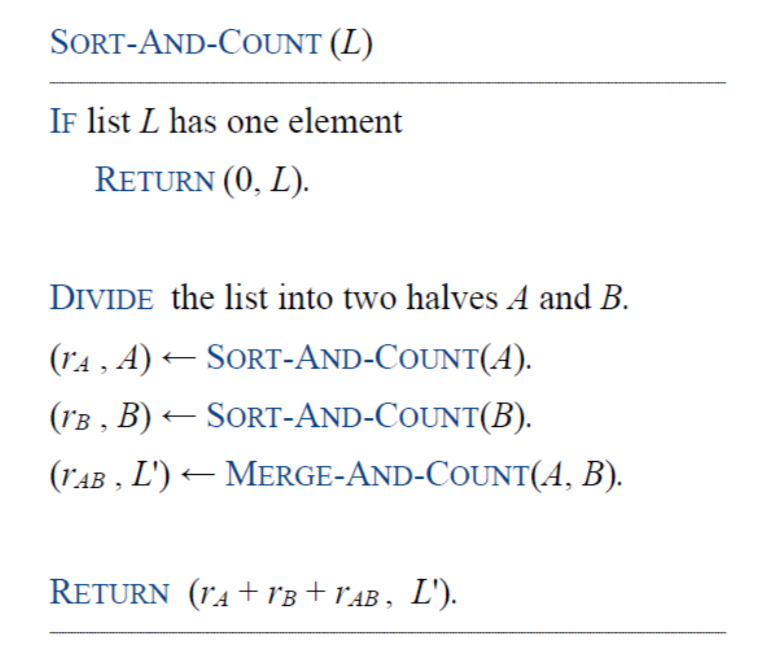
\includegraphics[scale=0.45]{p1}
\end{figure}

Count inversions $(a,b)$ with $a \in A$ and $b \in B$, assuming A and B are sorted:
\begin{enumerate}
	\item Scan A and B from left to right
	\item Compare $a_i$ and $b_j$
	\item If $a_i < b_j$, then $a_i$ is not inverted with any element left in B
	\item If $a_i > b_j$, then $b_j$ is inverted with every element left in A
	\item Append smaller element to sorted list C
\end{enumerate}

\paragraph{How do we formally prove correctness?}
\textcolor{red}{Induction on $n$} is usually very helpful, allows you to assume correctness of subproblems

\paragraph{Running time analysis}
$$T(n) = 2T(\frac{n}{2}) + O(n)$$
Master theorem says this is $T(n) = O(n \log n)$

\subsection{Closest Pair in $\real^2$}
\paragraph{Problem}
Given $n$ points of the form $(x_i, y_i)$ in the plane, find the closest pair of points.
\paragraph{Applications}
\begin{enumerate}
	\item Basic primitive in graphics and computer vision
	\item Geographic information systems, molecular modeling, air traffic control
	\item Special case of nearest neighbor
\end{enumerate}

\paragraph{Brute force running time}
$$\Theta(n^2)$$
\paragraph{Intuition from 1D?}
By sorting and checking, the problem would be easily $\mathcal{O}(n\log n)$
\paragraph{Non-degeneracy Assumption}
No two points have the same $x$ or $y$ coordinate
\paragraph{Closest Pair in $\real^2$}
\begin{enumerate}
	\item Divide: points in equal halves by drawing a vertical line L
	\item Conquer: solve each half recursively
	\item Combine: find closest pair with one point on each side of L
	\item Return the best of 3 solutions
\end{enumerate}

\under{Combine:} We can restrict our attention to points within $\epsilon$ of $L$ on each side, where $\epsilon$ = best of the solutions in two halves

\begin{figure}[h]
	\centering
	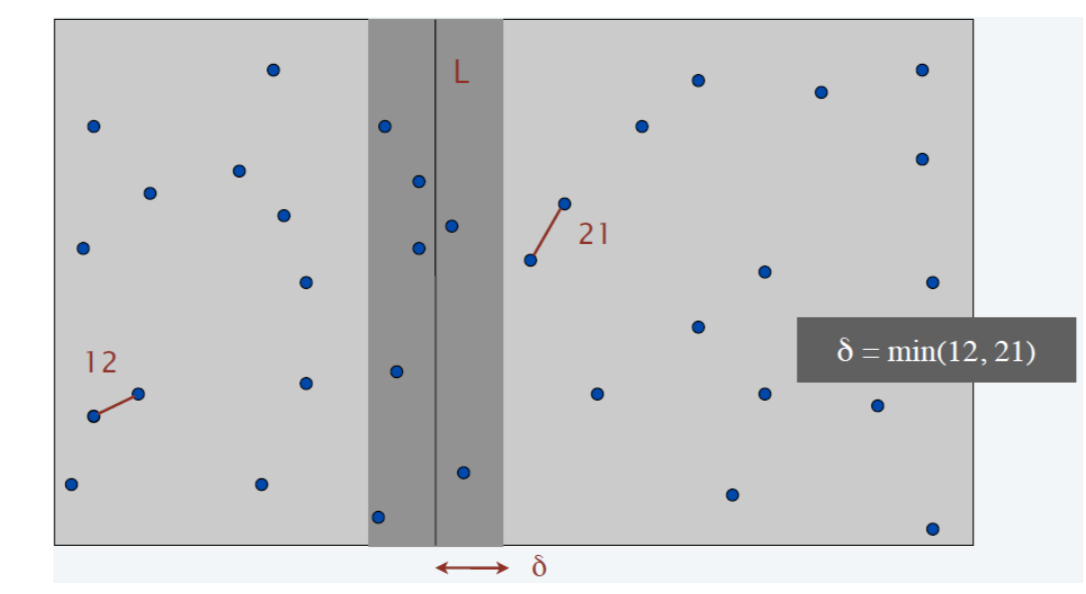
\includegraphics[scale=0.5]{p2}
\end{figure}

\begin{enumerate}
	\item Only need to look at points within $\epsilon$ of $L$ on each side
	\item Sort points on the strip by $y$ coordinate
	\item Only need to check each point with next \textcolor{red}{11} points in sorted list
\end{enumerate}
\paragraph{Why 11?}
Claim: If two points are at least 12 positions apart in the sorted list, their distance is at least $\epsilon$. \\
\proof \\
\begin{enumerate}
	\item No two points lie in the same $\delta / 2 \times \delta / 2$ box
	\item Two points that are more than two rows apart are at distance at least $\delta$
\end{enumerate}

\begin{figure}[h]
	\centering
	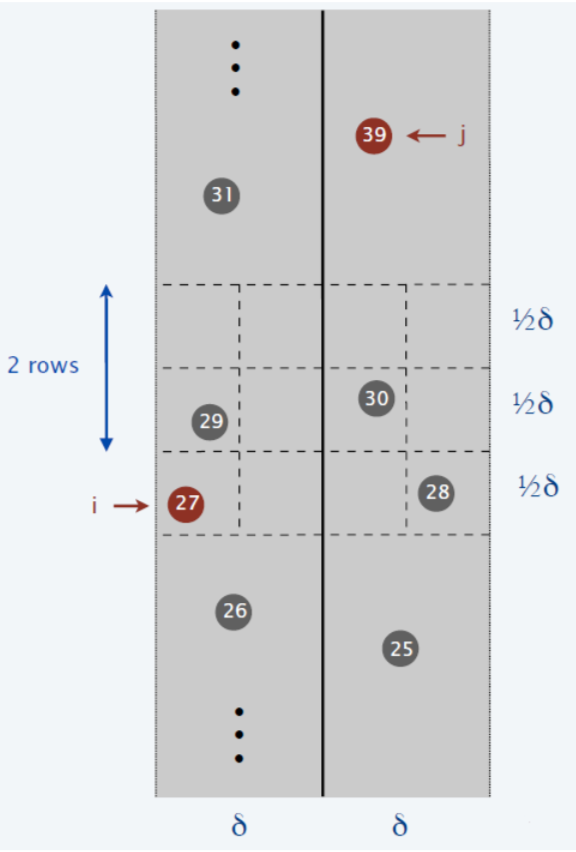
\includegraphics[scale=0.7]{p3}
\end{figure}

\subsection{Recap: Karatsuba's Algorithm}
Fast way to multiply two $n$ digit integers $x$ and $y$.
\paragraph{Brute force running time}
$\mathcal{O}(n^2)$

\paragraph{Algorithm}
\begin{enumerate}
	\item Divide each integer into two parts
	$$ x = x_1 * 10^{\frac{n}{2}} + x_2, y = y_1 * 10^{\frac{n}{2}} + y_2$$
	$$ xy = (x_1y_1) * 10^n + (x_1y_2 + x_2y_1) * 10^{\frac{n}{2}} + (x_2y_2)$$
	\item Four $\frac{n}{2}$-digit can be replaced by three
	$$x_1y_2 + x_2y_1 = (x_1 + x_2)(y_1 + y_2) - x_1y_1 - x_2y_2$$
\end{enumerate}

\paragraph{Running time}
$$T(n) = 3T(\frac{n}{2}) + \mathcal{O}(n)$$
$$\implies T(n) = \mathcal{O}(n^{\log_2{3}})$$

\subsection{Strassen's Algorithm}
Generalizes Karatsuba's insight to design a fast algorithm for multiplying two $n \times n$ matrices
$$ \begin{bmatrix} C_{11} & C_{12} \\
C_{21} & C_{22}
\end{bmatrix} 
= \begin{bmatrix} A_{11} & A_{12} \\
A_{21} & A_{22}
\end{bmatrix} * \begin{bmatrix} B_{11} & B_{12} \\
B_{21} & B_{22}
\end{bmatrix}$$
Call $n$ the ``size" of the problem. Naively, this requires 8 multiplications of size $\frac{n}{2}$, but by Strassen's insight, we can replace 8 multiplications by 7.\\
(Assume $n$ is a power of 2 because we need to recursively partition the matrix into 2-by-2 block matrices.)
\begin{figure}[h]
	\centering
	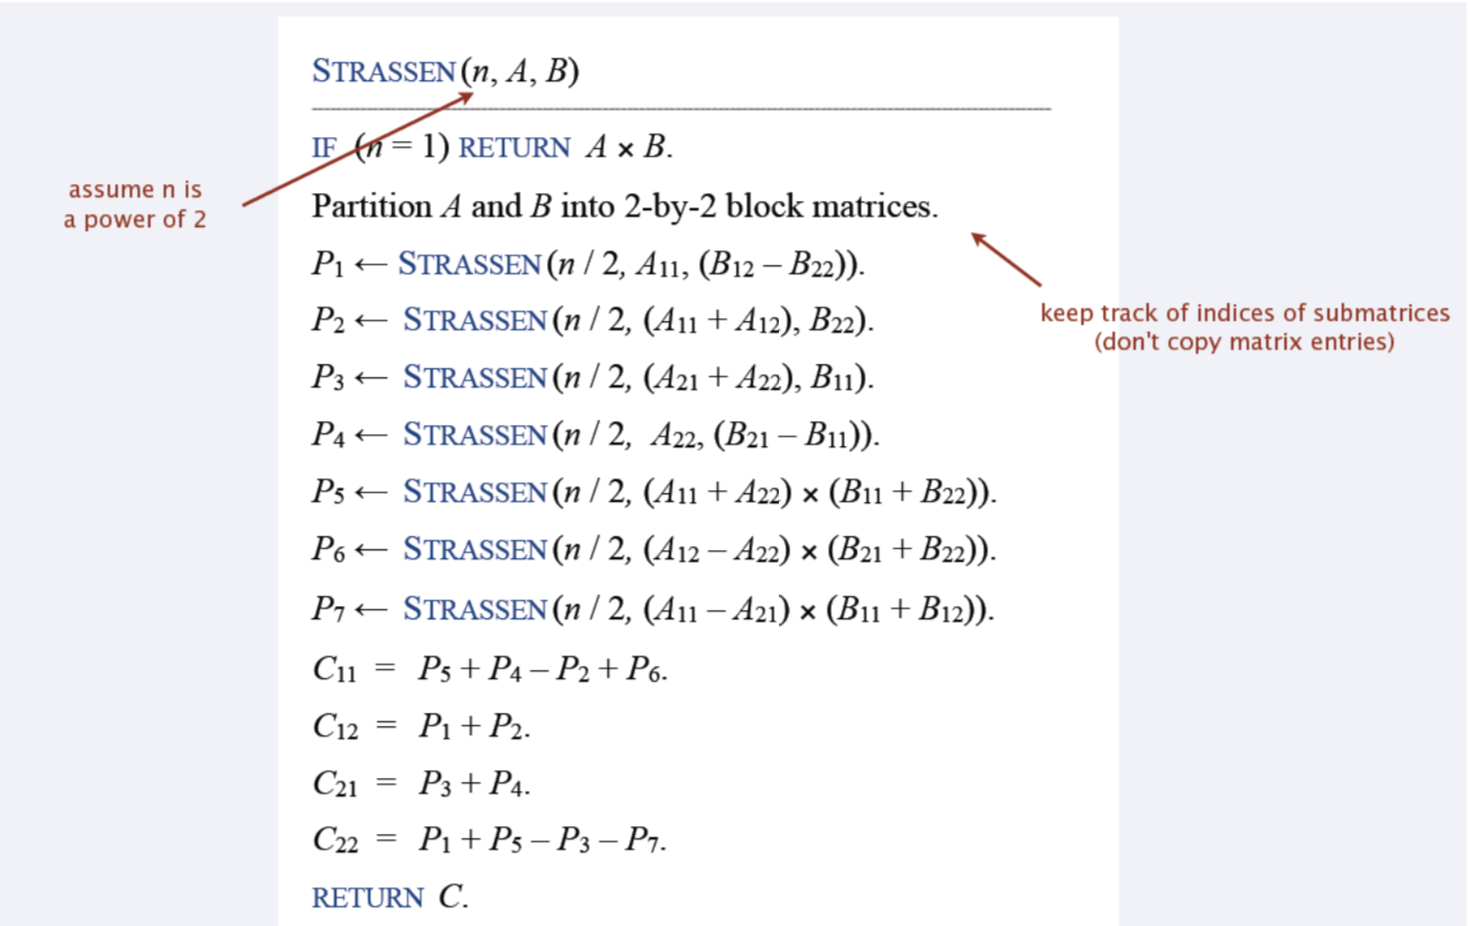
\includegraphics[scale=0.6]{p4}
\end{figure}

\paragraph{Running time}
$$T(n) = 7T(\frac{n}{2}) + \mathcal{O}(n^2)$$
$$T(n) \implies \mathcal{O}(n^{\log_2 7})$$


\subsection{Median \& Selection}
\paragraph{Selection}
Given $n$ comparable elements, find $k$th smallest. \\
\under{minimum}: $k$ = 1 \\
\under{maximum}: $k=n$ \\
\under{median}: $k = \lfloor (n+1) / 2\rfloor$

\paragraph{Different Implementations \& their running time}
\begin{enumerate}
	\item $\mathcal{O}(n)$ compares for min or max
	\item $\mathcal{O}(n \log n)$ compares by sorting
	\item $\mathcal{O}(n \log k)$ compares with a binary heap
\end{enumerate}

\paragraph{Applications}
\begin{enumerate}
	\item Order statistics
	\item ``top $k$"
	\item bottleneck paths
\end{enumerate}

\paragraph{Quick(Randomized) Select}
Selection is easier than sorting.
Partially sort array relative to a pivot element, and look for the $k$th smallest in subarray to the left or right of pivot.
\begin{figure}[h]
	\centering
	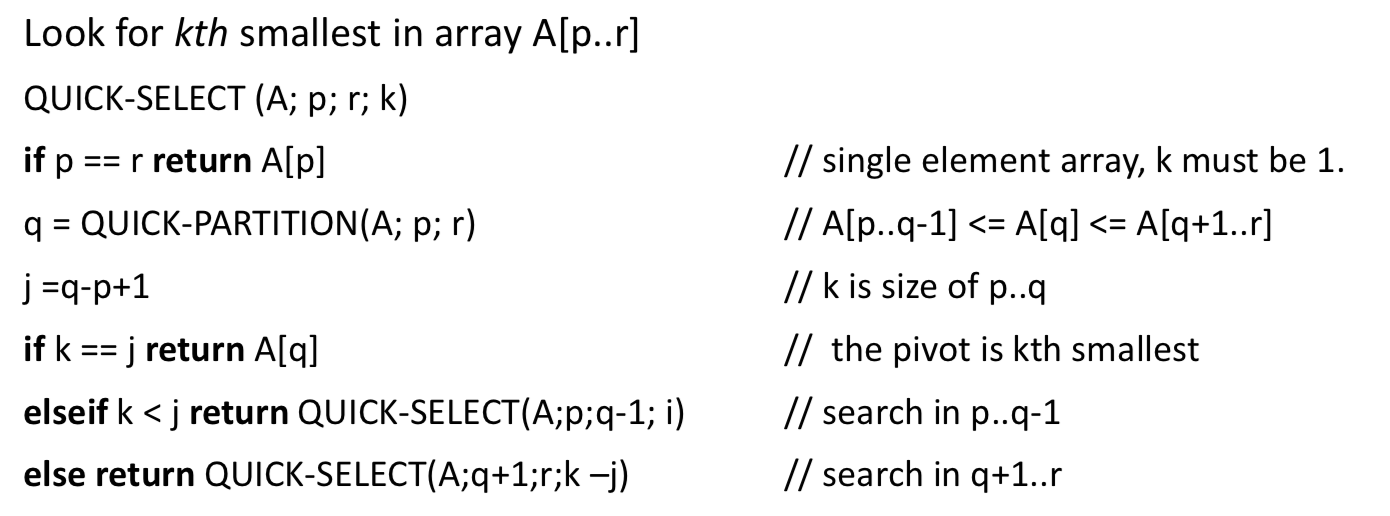
\includegraphics[scale=0.6]{p5}
\end{figure}
If partition only one element a time, then the algorithm would not be efficient. Therefore we need techniques to find a good pivot.

\paragraph{Finding a good pivot}
Algorithm as the following: \\
1. Divide $n$ elements into $\lfloor \frac{n}{5} \rfloor$ groups of 5 elements each (plus extra)\\
2. Find median of each group (except extra) 
\begin{figure}[h]
	\centering
	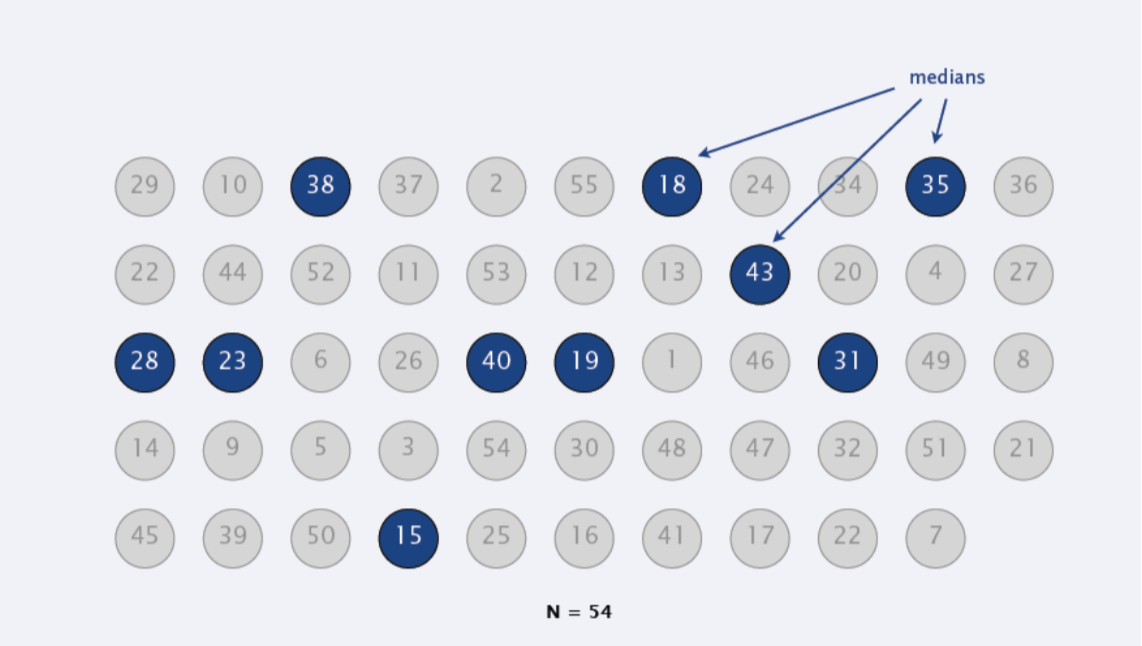
\includegraphics[scale=0.5]{p6}
\end{figure}

\noindent 3. Find median of medians recursively. \\
4. Use median-of-medians as pivot element.\\

\begin{figure}[h]
	\centering
	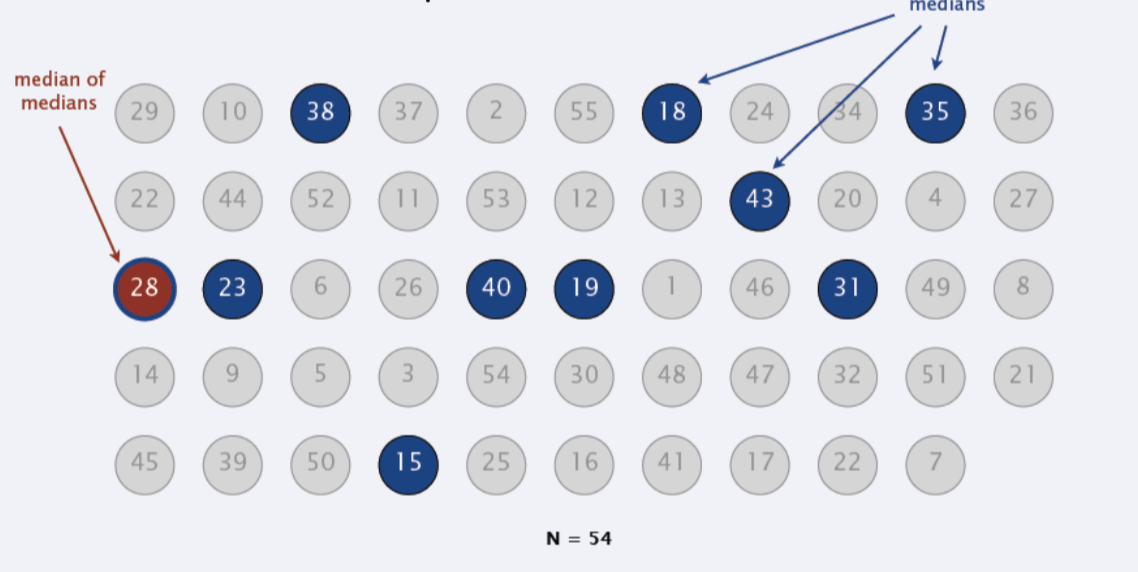
\includegraphics[scale=0.5]{p7}
\end{figure}

\paragraph{Analysis of median-of-medians selection algorithm - 5 element case}
\begin{enumerate}
	\item At least half of 5-element medians $\leq p$
	\item At least $\lfloor\lfloor n / 5 \rfloor / 2 \rfloor = \lfloor n / 10 \rfloor$ medians $\leq p$
	\item At least $3 \lfloor n / 10 \rfloor$ elements $\leq p$
	\item At least $3 \lfloor n / 10 \rfloor$ elements $\geq p$
	\item QUICK-SELECT() called recursively with at most $n - 3 \lfloor n / 10 \rfloor$ elements 
	\item \textcolor{blue}{[not clear]} $C(n) = $ max number of compares on an array of $n$ elements.
	$$C(n) \leq C(\lfloor \frac{n}{5} \rfloor) + C(n - 3\lfloor \frac{n}{10} \rfloor) + \frac{6}{5}n + n$$
	$\frac{6}{5}n$: we need 6 comparisons to find the median among 5 elements  \\
	$n$: cost of QUICK-PARTITION()
\end{enumerate}

\paragraph{Analysis of median-of-medians selection algorithm - general case}
\textcolor{blue}{[not clear]}
Suppose we have $m$ elements in each group. \\
Then we have approximately $\frac{n}{m}$ groups and $\frac{n}{2m}(1 + \frac{m-1}{2})$ number of elements less than median-of-medians. \\
Then $$T(n) = T(\frac{n}{m}) + T(n - \frac{n(m+1)}{4m}) $$
Want $$\frac{cn}{m} + cn > \frac{cn(m+1)}{4m}$$

$$\implies \frac{m+1}{4m} > \frac{1}{m} \implies m > 3$$
Choosing 4 involves floor and ceiling, so we choose 5 as the smallest number for which this algorithm can work.

\subsection{Algorithm Design}
Best algorithm for a problem is
\begin{enumerate}
	\item Typically hard to determine (We still don't know best algorithms for multiplying two $n$-digit integers or two $n \times n$ matrices)
	\item Usually, we design an algorithm and then analyze its running time, but some times we can do the reverse: \\
	E.g., if you know you want an $\mathcal{O}(n^2 \log n)$ algorithm, Master theorem suggests that you can get it by
	$$T(n) = 4T(\frac{n}{2}) + \mathcal{O}(n^2)$$
	So maybe you want to break your problem into 4 problems of size $\frac{n}{2}$ each, and then do $\mathcal{O}(n^2)$ computation to combine.
\end{enumerate}

\paragraph{Access to input}
For much of this analysis, we are assuming random access to elements of input, so we are ignoring underlying data structures (e.g. doubly linked list, binary tree, etc.)

\paragraph{Machine operations}
We're only counting comparison or arithmetic operations, so we are ignoring issues like how real numbers will be represented in closest pair problem. When we get to P vs NP, representation will matter.
\paragraph{Size of the problem}
Can be any reasonable parameter of the problem. For example, for matrix multiplication, we used $n$ as the size, while an input consists of two matrices with $n^2$ entries. It doesn't matter whether we call $n$ or $n^2$ the size of the problem, because the actual running time of the algorithm won't change.

\section{Greedy Algorithms}
\paragraph{Outline}
We want to find a solution $x$ that maximizes some objective function $f$, but the space of possible solutions $x$ is too large. Since the solution $x$ is typically composed of several parts (e.g. $x$ may be a set, composed of its elements), instead of directly computing $x$,
\begin{enumerate}
	\item Compute it one part at a time
	\item Select the next part ``greedily" to get maximum immediate benefit (\textcolor{red}{this needs to be defined carefully for each problem})
	\item May not be optimal because there is no foresight
	\item But sometimes this can be optimal too!
\end{enumerate}

\subsection{Interval Scheduling}
\paragraph{Problem}
Job $j$ starts at time $s_j$ and finishes at time $f_j$. Two jobs are compatible if they don't overlap. \\
\textcolor{red}{\under{Goal:}} find maximum-size subset of mutually compatible jobs

\paragraph{Greedy template}
Consider jobs in some ``natural" order. Take each job if it's compatible with the ones already chosen.

\paragraph{Order candidates}
\begin{enumerate}
	\item Earliest start time: ascending order of $s_j$
	\item Earliest finish time: ascending order of $f_j$
	\item Shortest interval: ascending order of $f_j - s_j$
	\item Fewest conflicts: ascending order of $c_j$, where $c_j$ is the number of remaining jobs that conflict with $j$
	\item Distance between jobs
\end{enumerate}

\paragraph{Counterexamples}
For proving 1,2,4 do not work:
\begin{figure}[h]
	\centering
	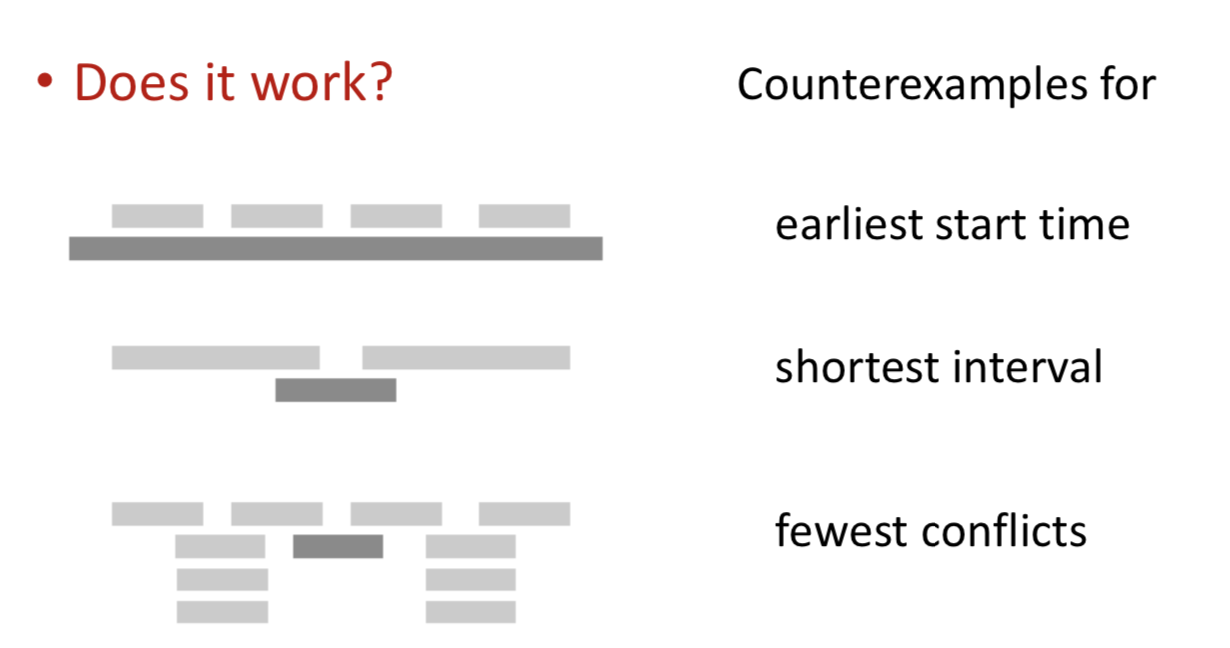
\includegraphics[scale=0.5]{p8}
\end{figure}

\paragraph{Implementing greedy with earliest finish time (EFT)}
Sort jobs by finish time. Say $f_1 \leq f_2 \leq \dots \leq f_n$. When deciding whether job $j$ should be included, we need to check whether it is compatible with all previously added jobs.\\
We only need to check if $s_j \geq f_{i^*}$, where $i^*$ is the last added job. This is because for any job $i$ added before $i^*, f_i \leq f_{i^*}$. So we can simply store and maintain the finish time of the last added job.
\paragraph{Running time}
$\mathcal{O}(n \log n)$ \\
(Sorting takes $n \log n$)

\paragraph{Optimality of greedy with EFT}
Suppose for contradiction that greedy is not optimal. \\
Say greedy selects jobs $i_1, i_2, \hdots, i_k$ sorted by finish time. \\
Consider the optimal solution $j_1, j_2, \hdots, j_m$ (also sorted by finish time) which matches greedy for as long as possible. That is, we want $j_1 = i_1, \hdots, j_r = i_r$ for greatest possible $r$.\\

\begin{figure}[h]
	\centering
	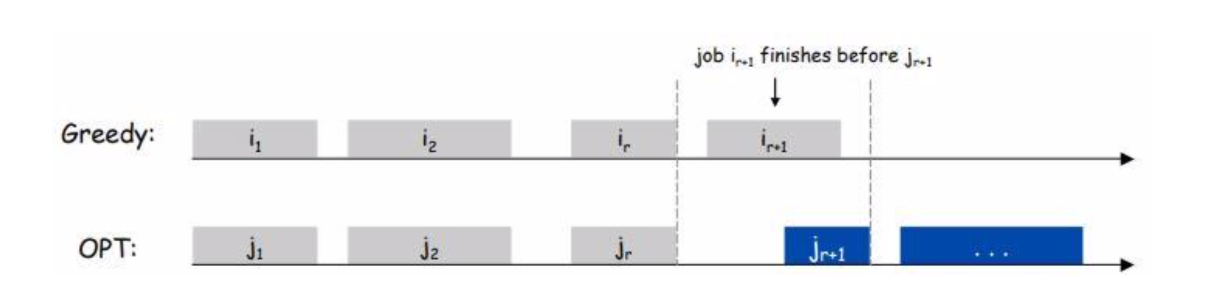
\includegraphics[scale=0.7]{p9}
\end{figure}

\noindent Both $i_{r+1}$ and $j_{r+1}$ were compatible with the previous selection ($i_1 = j_1, \hdots, i_r = j_r$)\\
Consider the solution $i_1, i_2, \hdots, i_r, i_{r+1}, j_{r+2}, \hdots, j_m$. It should still be feasible (\textcolor{red}{since $f_{i_{r+1}} \leq f_{j_{r+1}}$}), therefore it is still optimal, and it matches with greedy for one more step (contradiction!) \qed


\subsection{Interval Partitioning}
\paragraph{Problem}
Job $j$ starts at time $s_j$ and finishes at time $f_j$. Two jobs are compatible if they don't overlap.\\
\textcolor{red}{Goal:} group jobs into fewest partitions such that jobs in the same partition are compatible

\paragraph{One idea}
Find the maximum compatible set using the previous greedy EFT algorithm, call it one partition, recurse on the remaining jobs. \\
$\implies$ \textcolor{red}{Doesn't work!} \\

\noindent Think of scheduling lectures for various courses into few classrooms as possible.

\begin{figure}[h]
	\centering
	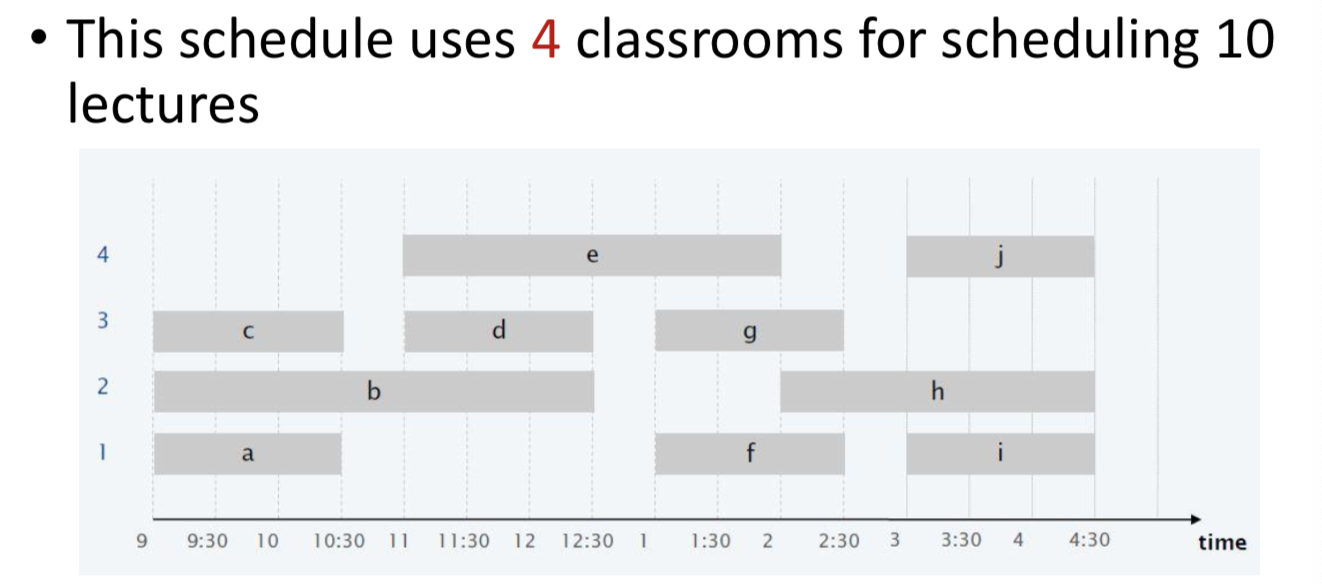
\includegraphics[scale=0.6]{p10}
\end{figure}

\begin{figure}[h]
	\centering
	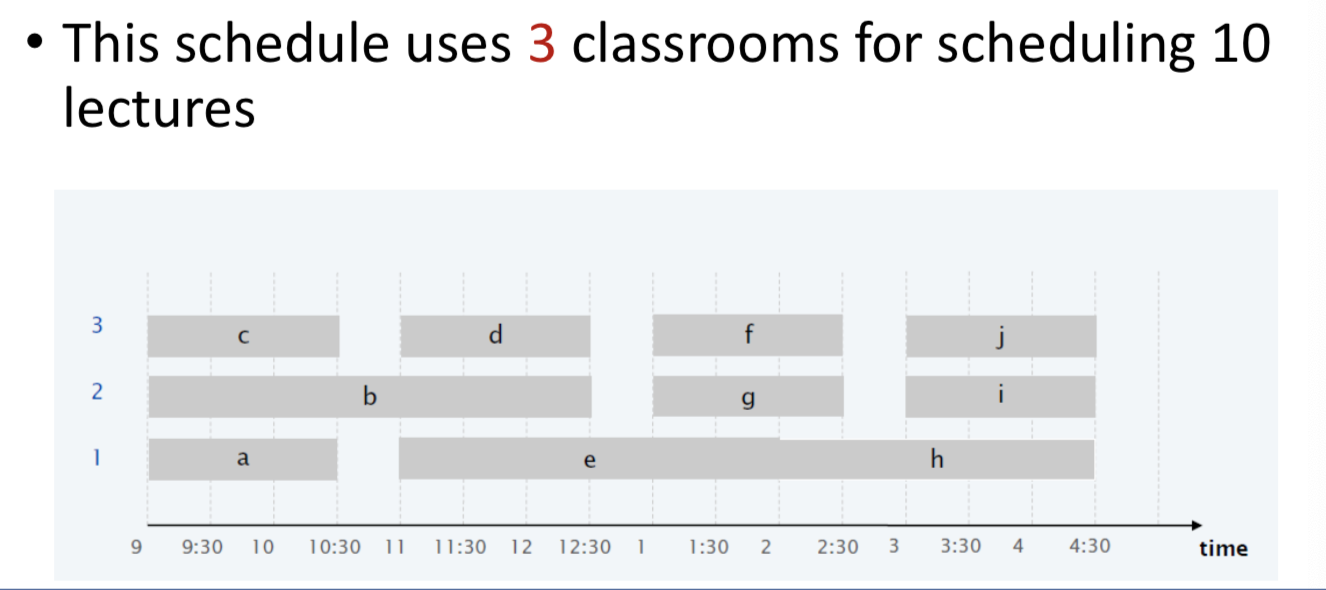
\includegraphics[scale=0.6]{p11}
\end{figure}

\paragraph{Greedy template}
Go through lectures in some ``natural order", assign each lecture to a compatible classroom, and \textcolor{red}{create a new classroom if the lecture conflicts with every existing classroom}

\paragraph{Order of lectures}
\begin{enumerate}
	\item Earliest start time: ascending order of $s_j$
	\item Earliest finish time: ascending order of $f_j$
	\item Shortest interval: ascending order of $f_j - s_j$
	\item Fewest conflicts: ascending order of $c_j$, where $c_j$ is the number of remaining jobs that conflict with $j$
\end{enumerate}


\begin{figure}[h]
	\centering
	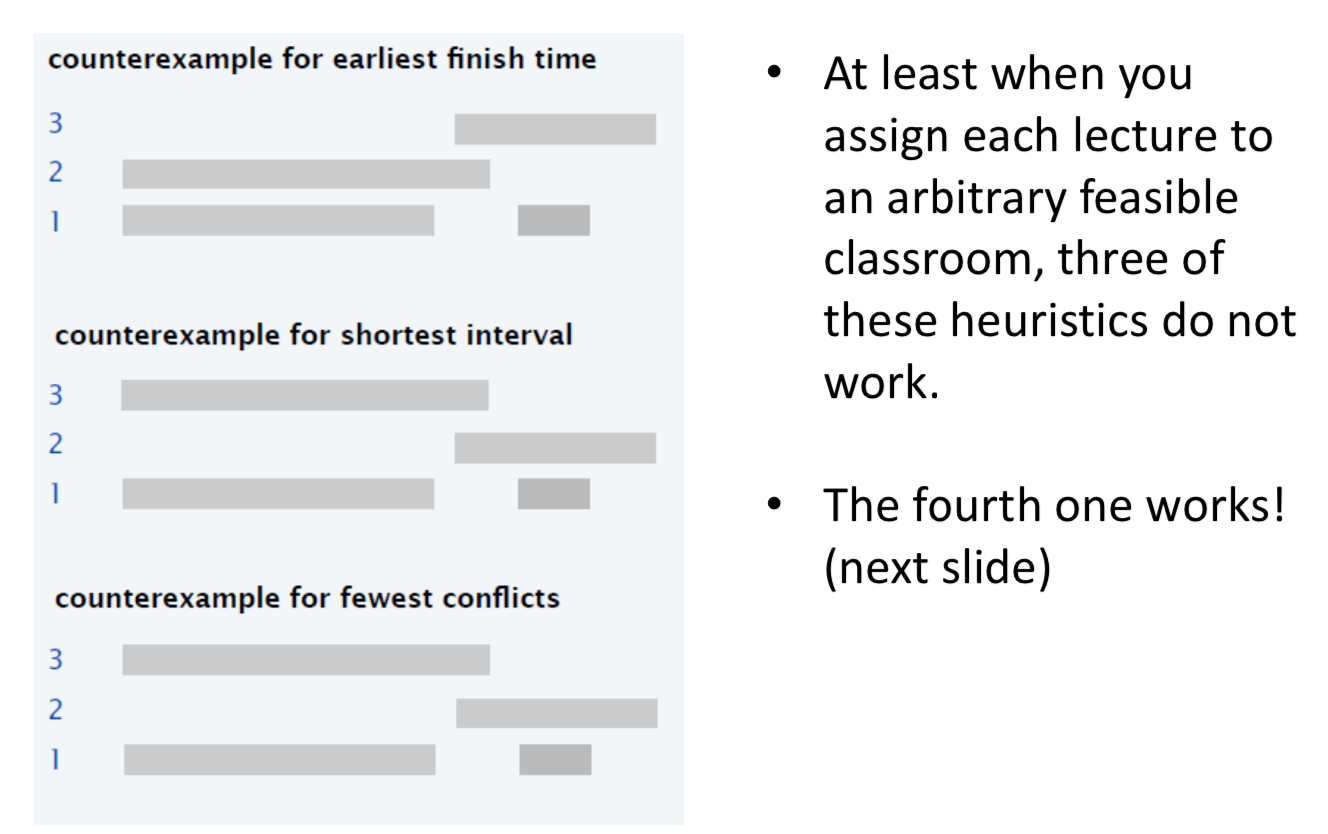
\includegraphics[scale=0.6]{p12}
	\caption{Counterexamples}
\end{figure}

\subsection{Interval Graphs}
Interval scheduling and interval partitioning can be seen as graph problems.
\paragraph{Input}
\begin{enumerate}
	\item Graph $G = (V, E)$
	\item Vertices $V = $ jobs or lectures
	\item Edge $(i, j) \in E$ if jobs $i$ and $j$ are incompatible
\end{enumerate}

\paragraph{Problems}
\begin{enumerate}
	\item Interval scheduling = \textcolor{red}{maximum independent set (MIS)}
	\item Interval partitioning = \textcolor{red}{graph colouring}
\end{enumerate}

\subsection{Minimizing Lateness}
\paragraph{Problem}
We have a single machine. Each job $j$ requires $t_j$ units of time and is due by time $d_j$. If it's scheduled to start as $s_j$, it will finish at $f_j = s_j + t_j$.\\
Lateness: $l_j = \max\{0, f_j - d_j\}$\\
\textcolor{red}{Goal:} minimize the maximum lateness, $L = \underset{j}{\max} \,l_j$ \\
Total lateness minimization is $NP-complete$

\paragraph{Contrast with interval scheduling}
\begin{enumerate}
	\item We can decide the start time
	\item All jobs must be scheduled on a single machine
\end{enumerate}

\subsection{Lossless Compression}
\paragraph{Problem}
We have a document that is written using $n$ distinct labels. \\
Naive encoding: represent each label using $k = \log n$ bits \\
If the document has length $m$, this used $m \log n$ bits. \\
But what if some labels are much more frequent in the document than others? We need to assign shorter codes to more frequent letters. \\
To avoid conflicts, we need \textcolor{red}{prefix-free encoding}: \\
Map each label $x$ to a bit-string $c(x)$ such that for all distinct labels $x$ and $y$, $c(x)$ is not a prefix of $c(y)$. So we can read left to right, find the first point where it becomes a valid encoding, decode the label, and continue.
\paragraph{Formal Problem}
Given $n$ symbols and their frequencies $(w_1, \hdots, w_n)$, find a prefix-free encoding with lengths $(l_1, \hdots, l_n)$ assigned to the symbols which minimizes $\sum_{i=1}^n w_i \cdot l_i$


\subsection{Other Greedy Algorithms}
\begin{enumerate}
	\item Dijkstra's shortest path algorithm
	\item Kruskal and Prim's minimum spanning tree algorithms
\end{enumerate}















\end{document}